\subsection{Response Surface Based Analysis}
\label{tutorial.uq.rs}

For simulation models that are expensive to run, response surface analysis can be a resourceful option. To construct a response surface, a space-filling sampling design is desired. For example, quasi-Monte Carlo (LPTAU) or Latin hypercube sampling schemes are recommended. Additionally, there are several possibilities for curve fitting methods. If the sample size is relatively small, polynomial regression or Gaussian process (if installed as part of PSUADE) is preferred. Alternatively, if the sample size is large enough (one hundred or more), cubic splines (if installed) may also be feasible.

\subsubsection{Response Surface Model Validation}

To proceed with response surface based analysis, the user needs to find a suitable response surface with which to approximate the input-to-output mapping. Validation is performed to see how well a particular response surface can predict a subset of the withheld data.
\begin{enumerate}
\item{Load ``lptau100\_10inputs\_4outputs.dat'' from the examples\bs UQ folder. Note: This is an extremely small simulation ensemble, as this is used to highlight the differences (in validation results) between a good response surface and a bad one.}
\item{Click \bu{Analyze} for the current ensemble. A new dialog page displays (Figure \ref{fig:uqt_rs_validate}).}
\item{Under ``Analysis'' (bottom section), under Step 1, select ``Response Surface.''
%%% INSERT: Analysis Screen, Response Surface Validation of Linear Model
\begin{figure}[H]
\centering 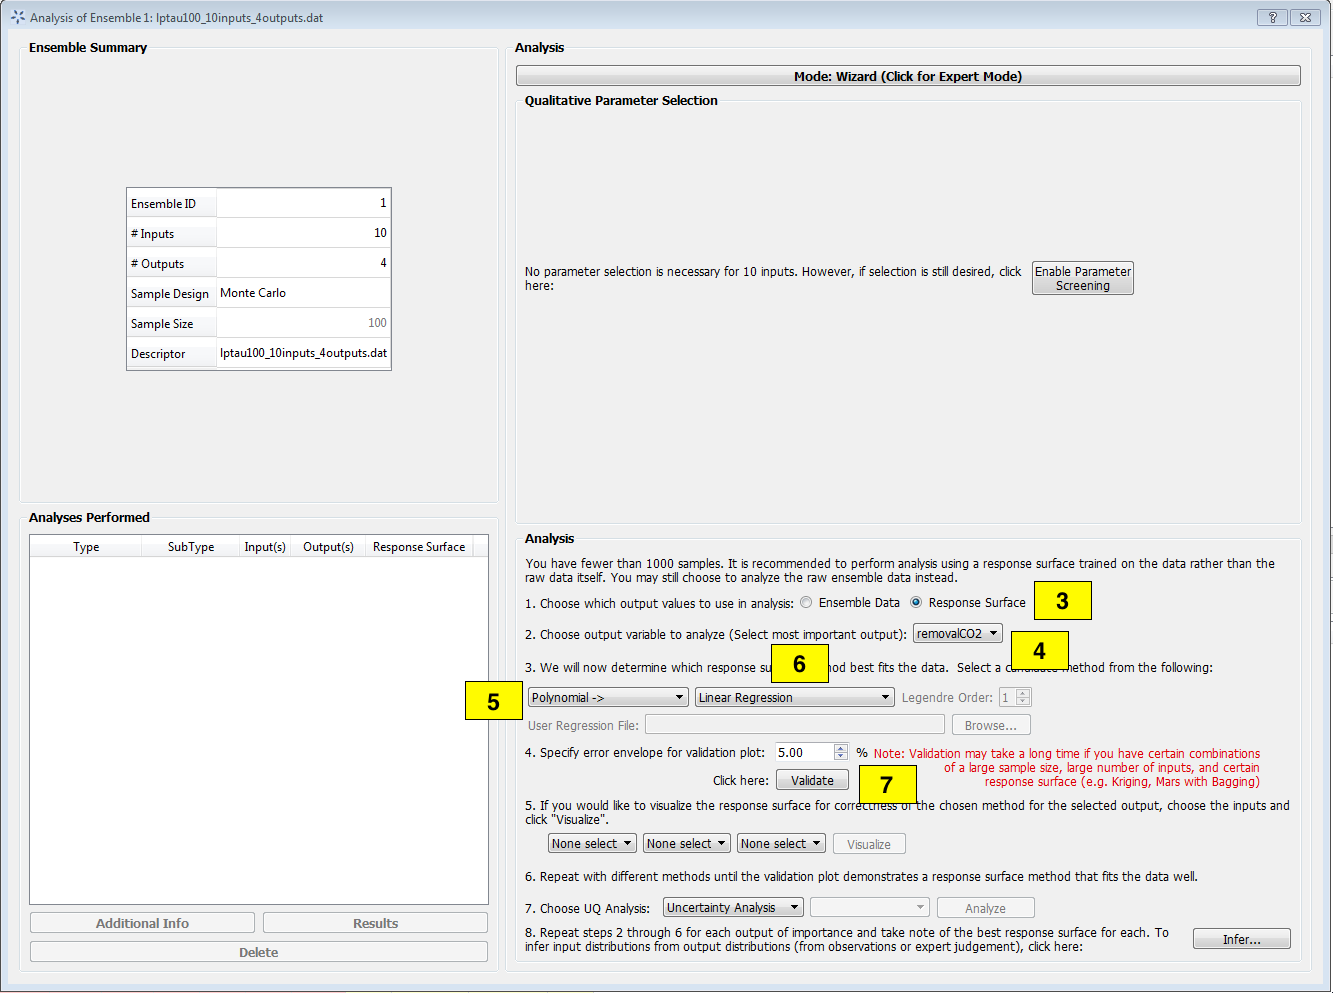
\includegraphics[width=6.5in,height=4in,keepaspectratio]{Chapt_uq/figs/tutorial/22_RSValidationScreen2}
\caption{Analysis Dialog, Response Surface Validation of Linear Model}
\label{fig:uqt_rs_validate}
\end{figure}
}
\item{Under Step 2, select ``removalCO2'' as the output for analysis.}
\item{Under Step 3, select ``Polynomial'' for response surface method.}
\item{There are multiple types of polynomial response surfaces, with increasing complexity as
the user navigates down the list. For now, select ``Linear'' in the next drop-down list.}
\item{Insert 5.00 as the error envelope for the validation plot. Click \bu{Validate}.  The result is illustrated in Figure \ref{fig:uqt_rs_validate_results}.}
\end{enumerate}

%%% INSERT: Linear Response Validation Results
\begin{figure}[H]
\centering 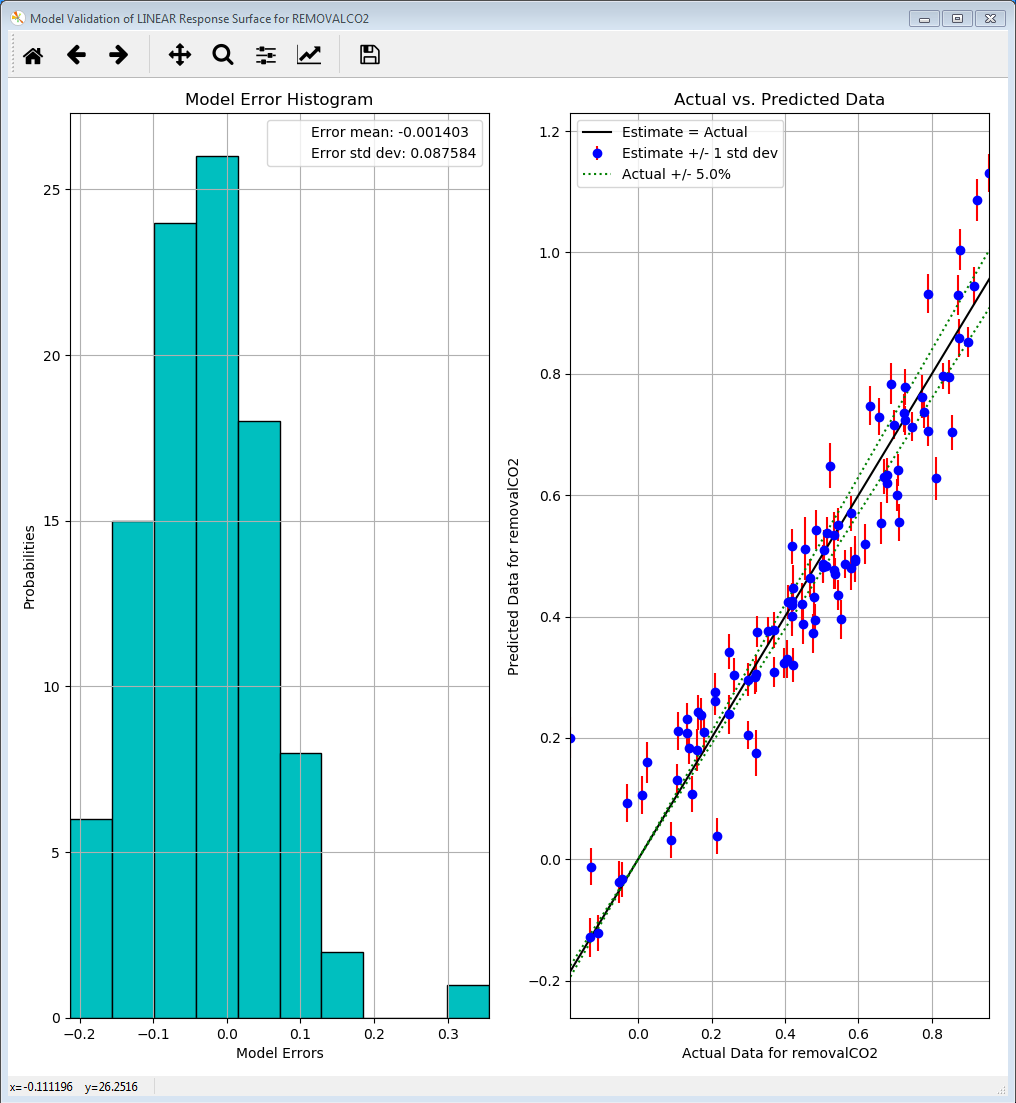
\includegraphics[width=6.5in,height=4in,keepaspectratio]{Chapt_uq/figs/tutorial/23_RSValidationLinear}
\caption{Linear Response Validation Results}
\label{fig:uqt_rs_validate_results}
\end{figure}

The cross-validation results for the linear regression model are displayed as a histogram of errors to the left and a plot of predicted values versus actual values to the right. The histogram displays the cross validation error distribution, which provides the user information on what the errors are like overall. If this distribution is not centered on zero, there may be a systematic bias in the response surface model. If the distribution is too wide, it is not a good fit. As for the plot of predicted values versus actual values, the more closely the points are to the diagonal, the better the fit. Most response surface models, with the exception of MARS, also provide
uncertainty information about the response surface. The vertical error bars on the left plot reflect the uncertainty in the linear response's predictions.

In summary, these two figures should provide sufficient information for the user to judge how good the fit is. As is apparent in the figures, the linear model consistently overestimates and thus is an ill-suited response surface to model our data. In general, the user may use a few response surface methods to see which method gives the best fit.

\subsubsection{Response Surface Based Uncertainty Analysis}

These capabilities are similar to those for ensemble data analysis. The difference is that the results are now derived from a much larger ensemble that is computed from the response surface. With the 100 samples from the ensemble data, a response surface is trained and is used to generate 100K samples internally to compute the results for uncertainty and sensitivity analyses. (Note: Validation must be performed before these analyses are available.)

After the response surface validation step, select ``Uncertainty Analysis''
to be the UQ analysis in Step 7 of ``Analysis'' (Figure
\ref{fig:uqt_rs_validate}). Click \bu{Analyze} and a distribution
representing the output uncertainty will be displayed (Figure \ref{fig:uqt_rsua_results}).

%%% INSERT: Response Surface Based Uncertainty Analysis Results
\begin{figure}[H]
\centering 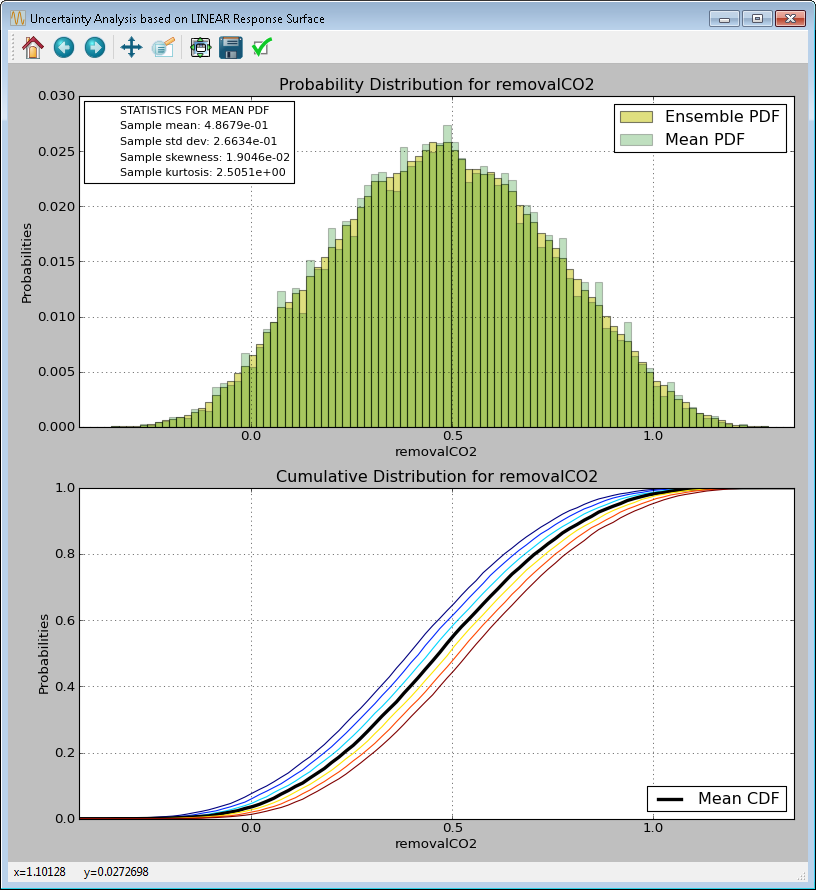
\includegraphics[width=6.5in,height=4in,keepaspectratio]{Chapt_uq/figs/tutorial/24_RSUAResults}
\caption{Response Surface Based Uncertainty Analysis Results}
\label{fig:uqt_rsua_results}
\end{figure}

Compare the response surface based uncertainty results (Figure \ref{fig:uqt_rsua_results}) to the results from ensemble data analysis (Figure \ref{fig:uqt_ua_results}). The two main differences are easily seen.

\begin{itemize}
\item{{\bf Two PDFs on top plot:} A response surface (in this case, linear regression) is used to predict the output values corresponding to the input samples. From the validation step (left plot of Figure \ref{fig:uqt_rs_validate_results}). Note: There is error associated with the response surface’s predictions. This error is propagated in uncertainty analysis, in the form of standard deviations around the predicted output values (i.e., the means). \\
	
	Accordingly, two histograms are presented: The ``mean PDF'' represents the output probability distribution computed from the response surface's predicted output values only, without consideration for the uncertainties surrounding these predicted values. The ``ensemble PDF'' represents the output probability distribution that encompasses the uncertainties surrounding these predicted values. In most cases, the ensemble PDF should have a larger spread because it is accounting for more uncertainties (i.e., those that stem from the approximations inherent in the response surface).}
\item{{\bf Multiple cumulative distribution functions (CDFs) on bottom plot:} The ``mean CDF'' is constructed from a cumulative sum on the mean PDF in the top plot. Since each predicted output value (i.e., the mean) has an associated standard deviation, this information is used to construct other PDFs that correspond to output values that are +/- 1, 2, and 3 standard deviations from the mean. These PDFs are then converted to CDFs and shown as colored lines. These colored lines provide an uncertainty ``envelope'' around the mean CDF.}
\end{itemize}

\subsubsection{Response Surface Based Mixed Epistemic-Aleatory Uncertainty Analysis}

In ``Expert Mode'', the user can perform more advanced uncertainty analysis
that handles both epistemic and aleatory uncertainties.
To do so, the user will need to designate the uncertainty type (epistemic or
aleatory) for each uncertain input. In general, epistemic uncertainties are
reducible uncertainties that arise due to lack of knowledge, such as
simplifying assumptions in a mathematical model. Therefore, epistemic
uncertainty is
often characterized by upper and lower bounds. On the other hand, aleatory
uncertainties are irreducible uncertainties that represent natural,
physical variability in the phenomenon under study. As such, aleatory
uncertainties are often characterized by distributions. Hence, the user is
required to provide a PDF for each aleatory input.
(In FOQUS, with the exception of mixed epistemic-aleatory uncertainty
analysis, all uncertain inputs are treated as aleatory inputs.)

To perform mixed epistemic-aleatory uncertainty (Figure
\ref{fig:uqt_rsaeua}), switch to ``Expert Mode''
by clicking the \bu{Mode} button that toggles between the analysis
modes. After response surface validation, select ``Uncertainty Analysis''
in the first \textbf{\underline{Choose UQ Analysis}} drop-down list, then ``Epistemic-Aleatory'' in the secondary
drop-down list, for the UQ analysis. In the input table, designate the
parameter \textbf{\underline{Type}} (``Epistemic'', ``Aleatory'' or ``Fixed'') and the corresponding
information for each input. Once complete, click \textbf{\underline{Analyze}}.

%%% INSERT: Response Surface Based Mixed Epistemic-Aleatory Uncertainty Analysis
\begin{figure}[H]
\centering
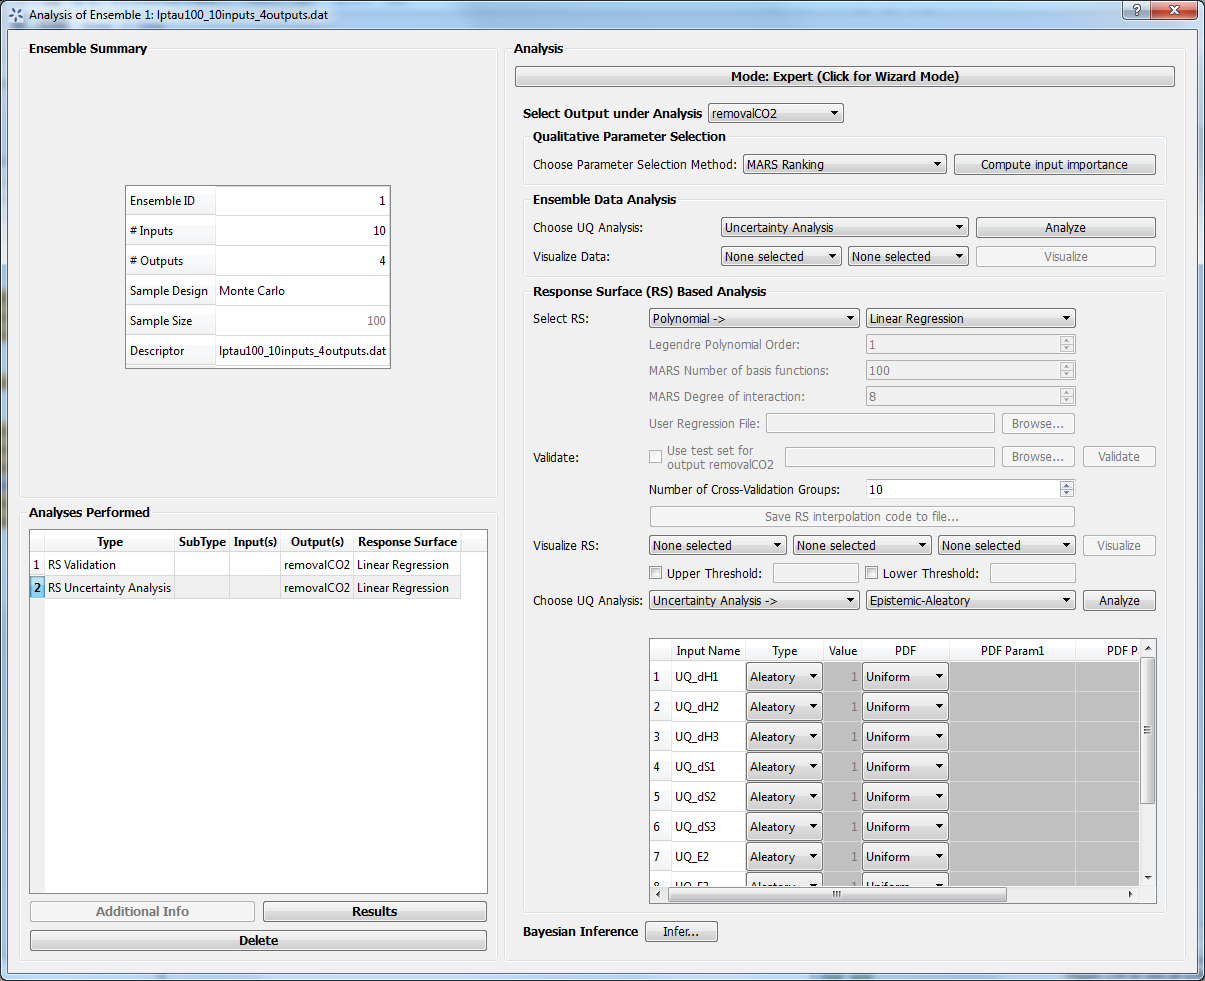
\includegraphics[width=6.5in,height=4in,keepaspectratio]{Chapt_uq/figs/tutorial/24a_RSAEUA}
\caption{Response Surface Based Mixed Epistemic-Aleatory Uncertainty Analysis}
\label{fig:uqt_rsaeua}
\end{figure}

The results of mixed epistemic-aleatory uncertainty analysis is a plot
(Figure \ref{fig:uqt_rsaeua_results})
containing multiple CDFs. In the mixed analysis, the epistemic inputs are
sampled according to their lower and upper bounds. Each sample point spawns
a response surface based uncertainty analysis, in which 
the epistemic inputs are fixed at their sampled value and the aleatory
input uncertainties are propagated to generate a CDF that represents the
output uncertainty. A slider is provided for the user to extract the
probability range corresponding to a particular value of the output.

%%% INSERT: Response Surface Based Mixed Epistemic-Aleatory Uncertainty Analysis Results
\begin{figure}[H]
\centering 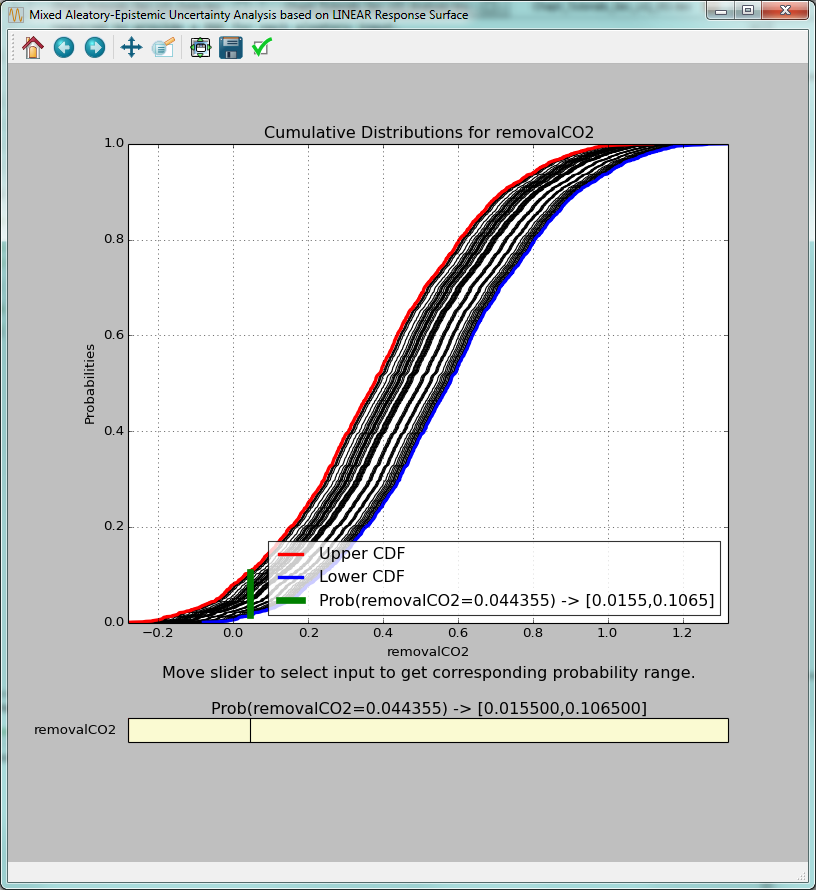
\includegraphics[width=6.5in,height=4in,keepaspectratio]{Chapt_uq/figs/tutorial/24b_RSAEUAResults}
\caption{Response Surface Based Mixed Epistemic-Aleatory Uncertainty Analysis Results}
\label{fig:uqt_rsaeua_results}
\end{figure}

\subsubsection{Response Surface Based Sensitivity Analysis}

For quantitative sensitivity analysis, follows these steps:
\begin{enumerate}
\item{In the \textbf{\underline{Choose UQ Analysis}} drop-down list (Step 6 of ``Analysis''), select ``Sensitivity Analysis.''}
\item{In the next drop-down list, select ``First-order'' and click \bu{Analyze}. (This analysis may
take a long time depending on the sample size and the response surface used.)}
\end{enumerate}
Prediction errors are associated with the response surface's predictions of the output values (left plot of Figure \ref{fig:uqt_rs_validate_results}). Earlier, it was observed that the response surface error contributed to the output uncertainty, leading to a larger spread in the output PDF (top plot of Figure \ref{fig:uqt_rsua_results}). In Figure \ref{fig:uqt_rssa_results}, the response surface error contributed to uncertainty (shown as blue error bars) surrounding each input's contribution to the output variance (shown as yellow bars).

%%% INSERT: Response Surface Based First-order Sensitivity Results
\begin{figure}[H]
	\centering \includegraphics[width=6.5in,height=4in,keepaspectratio]{Chapt_uq/figs/tutorial/25_RSSobol1Results}
	\caption{Response Surface Based First-order Sensitivity Results}
	\label{fig:uqt_rssa_results}
\end{figure}

\subsubsection{Response Surface Based Visualization}

The response surface that has been validated can also be visualized.

\begin{enumerate}
\item{Select one input next to ``Visualize Response Surface.''}
\item{Click \bu{Visualize} to display a 2-D line plot that displays ``removalCO2'' versus the selected
input.
%%% INSERT: 1-D Response Surface Visualization 
\begin{figure}[H]
\centering 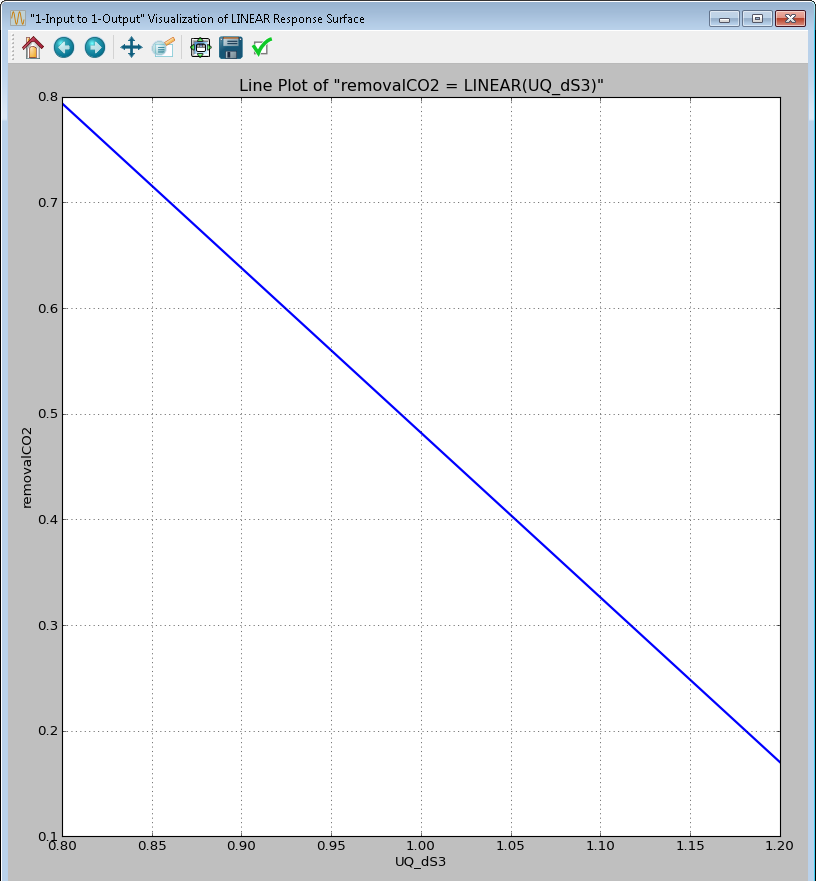
\includegraphics[width=6.5in,height=4in,keepaspectratio]{Chapt_uq/figs/tutorial/26_1DRSVis}
\caption{1-D Response Surface Visualization }
\label{fig:uqt_rs1_results}
\end{figure}
}
\item{Select another input next to the first one for a 2-D response surface visualization.}
\item{Click \bu{Visualize} to display a figure with a 3-D surface plot and a 2-D contour plot (Figure \ref{fig:uqt_rs2_results}).\\
%%% INSERT: 2-D Response Surface Visualization 
\begin{figure}[H]
\centering \includegraphics[width=6.5in,height=4in,keepaspectratio]{Chapt_uq/figs/tutorial/27_2DRSVis}
\caption{2-D Response Surface Visualization }
\label{fig:uqt_rs2_results}
\end{figure}
}
\item{Select another input next to the second one for a 3-D response surface visualization.}
\item{Click \bu{Visualize} to display a 3-D isosurface plot. Move the slider to see the points in the 3-D input space that fall within the small range of ``removalCO2'' (Figure \ref{fig:uqt_rs3_results}).
%%% INSERT: 3-D Response Surface Visualization 
\begin{figure}[H]
\centering 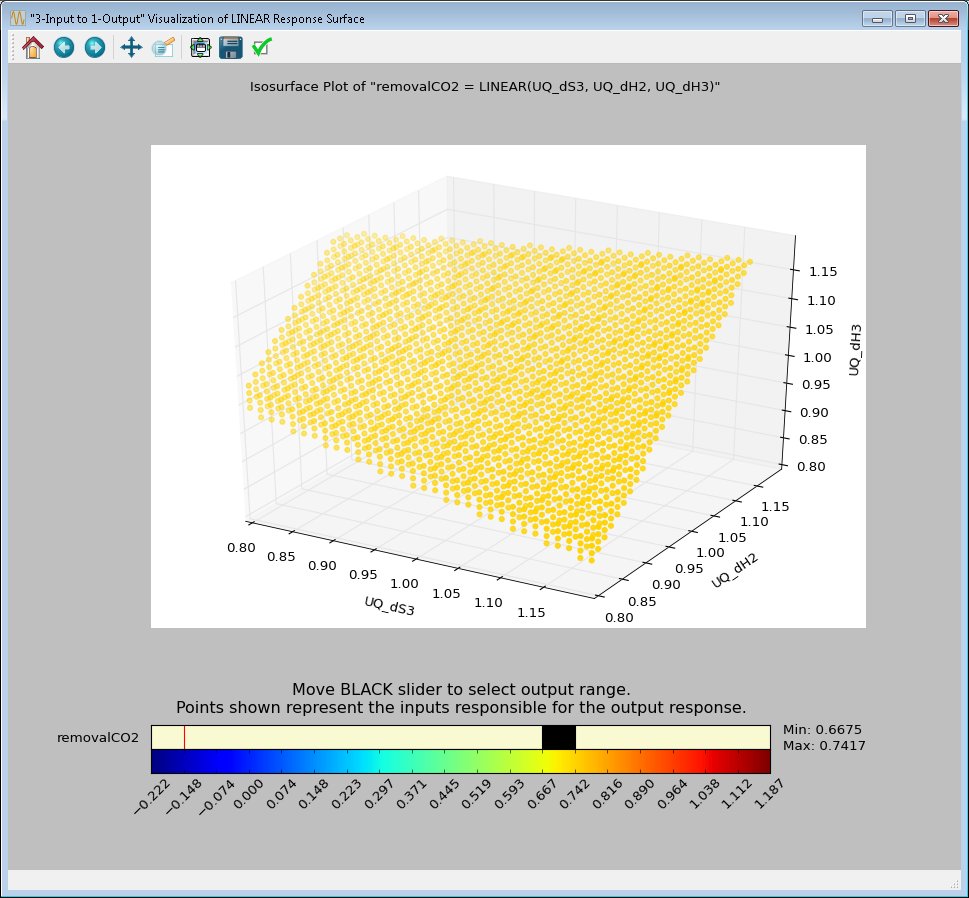
\includegraphics[width=6.5in,height=4in,keepaspectratio]{Chapt_uq/figs/tutorial/28_3DRSVis}
\caption{3-D Response Surface Visualization }
\label{fig:uqt_rs3_results}
\end{figure}
}
\end{enumerate}
